\documentclass[14pt]{beamer}

\usepackage[utf8]{inputenc}
\usepackage[T1]{fontenc}
\usepackage{tikz}
\usepackage{xcolor}
\usepackage{minted}
\usepackage{graphicx}
\usepackage{amssymb}
\usepackage{bussproofs}

\usetikzlibrary{shapes.geometric,arrows}

\tikzstyle{startstop} = [rectangle, rounded corners, text centered, draw=black]
\tikzstyle{io} = [trapezium, trapezium left angle=70, trapezium right angle=110, text centered, draw=black]
\tikzstyle{process} = [rectangle, text centered, draw=black]
\tikzstyle{decision} = [diamond, aspect=2, text centered, draw=black]
\tikzstyle{arrow} = [thick,->,>=stealth]

\title{Extensional crisis and proving identity}

\author{Ashutosh Gupta, Laura Kovács, Bernhard Kragl, Andrei~Voronkov\\ presented by Simon Robillard and Nikita Frolov}
\institute{}
\date{}

\beamertemplatenavigationsymbolsempty
\useoutertheme{infolines}

\begin{document}

\begin{frame}
  \maketitle
\end{frame}

\section{Motivating examples}
\begin{frame}{A simple problem in set theory}
  Prove that set union is commutative
  \[
  \forall a \; b,\; a \cup b = b \cup a
  \]

  The following two axioms are used in the proof
  \begin{itemize}
  \item Definition of union
    \[
    \forall a \; b\; e,\; e \in a \cup b \leftrightarrow e \in a \lor e \in b
    \]
  \item Extensionality
    \[
    \forall a \; b,\; (\forall e,\; e \in a \leftrightarrow e \in b) \rightarrow a = b
    \]
  \end{itemize}
\end{frame}

\begin{frame}{A closer look at the extensionality axiom}
  \[
  \begin{array}{rc}
    & \forall a \; b,\; (\forall e,\; e \in a \leftrightarrow e \in b) \rightarrow a = b \\
    & \\
    \uncover<2->{\textcolor{gray}{\equiv} & \textcolor{gray}{\text{\{ skolemization \}}}} \\
    & \\
    & \uncover<2->{(sk(x, y) \in x \not\leftrightarrow sk(x, y) \in y) \lor x = y} \\
    & \\
    \uncover<3->{\textcolor{gray}{\equiv} & \textcolor{gray}{\text{\{ CNF transformation \}}}} \\
    & \\
    \uncover<3->{& sk(x, y) \in x \lor sk(x, y) \in y \lor x = y} \\
    & \uncover<3->{\land} \\
    & \uncover<3->{sk(x, y) \not\in x \lor sk(x, y) \not\in y \lor x = y}
  \end{array}
  \]
\end{frame}

\begin{frame}{Selection on extensionality clauses}
  \[
  sk(x, y) \not\in x \lor sk(x, y) \not\in y \lor x = y
  \]

  The literal $x = y$ is
  \begin{itemize}
  \item positive
  \item always the smallest literal 
  \end{itemize}
\end{frame}

\begin{frame}{Direction of search}
  We want to use the goal for superposition
  \begin{prooftree}
    \AxiomC{$A \lor \underline{x = y}$}
    \AxiomC{$\underline{s \neq t}$}
    \BinaryInfC{$A\theta$}
  \end{prooftree}
  But instead we can only superpose
  \begin{prooftree}
    \AxiomC{$\underline{A} \lor x = y$}
    \AxiomC{$\underline{\neg A'} \lor B$}
    \BinaryInfC{$(x = y \lor B)\theta$}
  \end{prooftree}
\end{frame}

\begin{frame}{Solutions?}
  \begin{itemize}
  \item Select only $x = y$? Loss of completeness
  \item Select it in addition to other literals
  \end{itemize}
  
  {\footnotesize
    \begin{prooftree}
      \AxiomC{$\underline{x = y} \lor sk(x, y) \not\in x \lor sk(x, y) \not\in y$}
      \AxiomC{$\underline{e \not\in x \cup y} \lor e \in x \lor e \in y$}
      \BinaryInfC{$sk(x \cup y, z) \not\in x \cup y \lor sk(x \cup y, z) \not\in z \lor e \not\in x \cup y \lor e \in x \lor e \in y$}
    \end{prooftree}
  }
\end{frame}


\section{Extensionality resolution}
\begin{frame}{Extensionality resolution rule}
  \begin{prooftree}
    \AxiomC{$x = y \lor C$}
    \AxiomC{$s \neq t \lor D$}
    \BinaryInfC{$C \theta \lor D$}
  \end{prooftree}

  where

  \begin{itemize}
  \item $ext\_rec(x = y \lor C) = (x = y)$
    
    \begin{itemize}
    \item $ext\_rec$ is undefined for clauses without equalities
    \item $ext\_rec$ is defined for \emph{extensionality clauses}
    \end{itemize}
    
  \item $s \neq t$ is selected in $s \neq t \lor D$
  \item $\theta = \{ x \mapsto s, y \mapsto t \}$
  \end{itemize}
\end{frame}

\begin{frame}{Soundness of extensionality resolution}
  \begin{prooftree}
    \AxiomC{$\neg C \to x = y$}
    \AxiomC{$s = t \to D$}
    \BinaryInfC{$\neg {C \theta} \to D$}
  \end{prooftree}
\end{frame}


\begin{frame}{Otter saturation algorithm}
  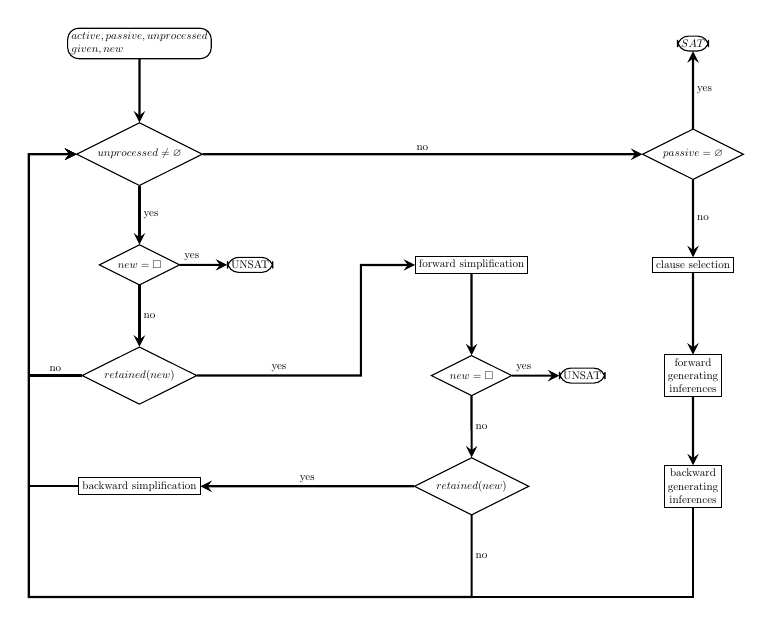
\begin{tikzpicture}[node distance=100, scale=0.4, every node/.style={transform shape}]
    \node (input) [startstop, align=left] {$active, passive, unprocessed$ \\ $given, new$};

    \node (nounprocessed) [decision, below of=input] {$unprocessed \neq \varnothing$};
    \node (newemptyclause) [decision, below of=nounprocessed] {$new = \square$};
    \node (retainednew) [decision, below of=newemptyclause] {$retained(new)$};
    \node (unsat) [startstop, right of=newemptyclause] {UNSAT};

    \coordinate[left of=newemptyclause]  (1);
    \coordinate[right of=unsat] (2);

    \node (forwardsimplification) [process, right of=2] {forward simplification};
    \node (newemptyclause2) [decision, below of=forwardsimplification] {$new = \square$};
    \node (retainednew2) [decision, below of=newemptyclause2] {$retained(new)$};
    \node (unsat2) [startstop, right of=newemptyclause2] {UNSAT};
    \node (backwardsimplification) [process, below of=retainednew] {backward simplification};

    \node (forwardinference) [process, right of=unsat2, align=center] {forward \\ generating \\ inferences};
    \node (backwardinference) [process, below of=forwardinference, align=center] {backward \\ generating \\ inferences};
    \node (clauseselection) [process, above of=forwardinference] {clause selection};
    \node (nopassive) [decision, above of=clauseselection] {$passive = \varnothing$};
    \node (sat) [startstop, above of=nopassive] {$SAT$};

    \coordinate[below of=retainednew2] (3);

    \draw [arrow] (input) -- (nounprocessed);
    \draw [arrow] (nounprocessed) -- node [right] {yes} (newemptyclause);
    \draw [arrow] (newemptyclause) -- node [right] {no} (retainednew);
    \draw [arrow] (newemptyclause) -- node [near start, above] {yes} (unsat);
    \draw [arrow] (retainednew) -| node [near start, above] {no} (1) |- (nounprocessed);
    \draw [arrow] (retainednew) -| node [near start, above] {yes} (2) -- (forwardsimplification);
    \draw [arrow] (forwardsimplification) -- (newemptyclause2);
    \draw [arrow] (newemptyclause2) -- node [right] {no} (retainednew2);
    \draw [arrow] (newemptyclause2) -- node [near start, above] {yes} (unsat2);
    \draw [arrow] (retainednew2) -- node [right] {no} (3) -| (1) |- (nounprocessed);
    \draw [arrow] (retainednew2) -- node [midway, above] {yes} (backwardsimplification);
    \draw [arrow] (backwardsimplification) -| (1) |- (nounprocessed);

    \draw [arrow] (nounprocessed) -- node [midway, above] {no} (nopassive);
    \draw [arrow] (nopassive) -- node [right] {no} (clauseselection);
    \draw [arrow] (nopassive) -- node [right] {yes} (sat);
    \draw [arrow] (clauseselection) -- (forwardinference);
    \draw [arrow] (forwardinference) -- (backwardinference);
    \draw [arrow] (backwardinference) |- (3) -| (1) |- (nounprocessed);
  \end{tikzpicture}
\end{frame}

\begin{frame}{...with extensionality resolution}
  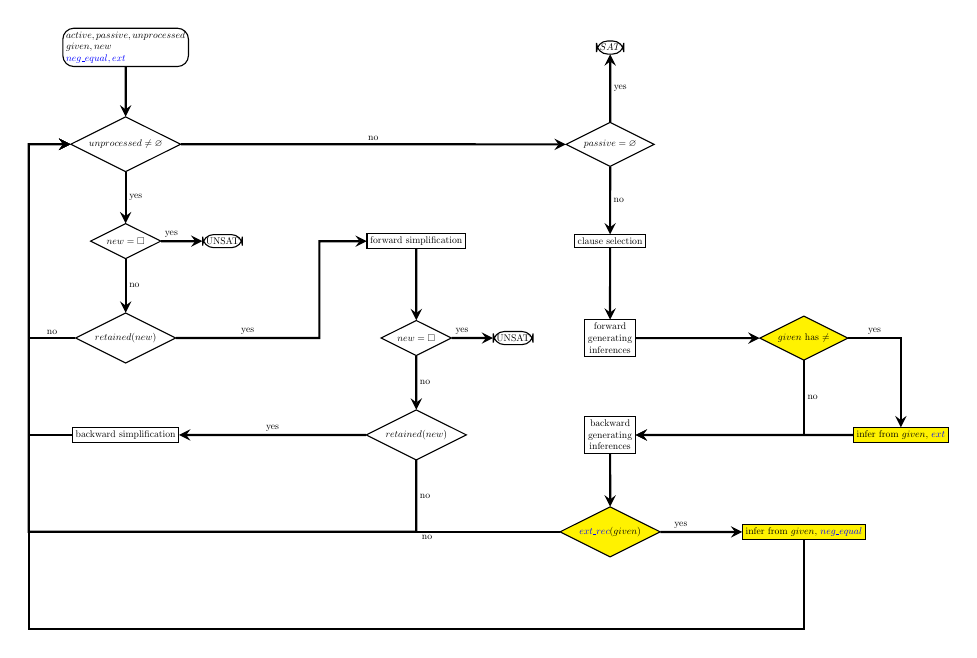
\begin{tikzpicture}[node distance=100, scale=0.35, every node/.style={transform shape}]
    \node (input) [startstop, align=left] {$active, passive, unprocessed$ \\ $given, new$ \\ \textcolor{blue}{$neg\_equal, ext$}};

    \node (nounprocessed) [decision, below of=input] {$unprocessed \neq \varnothing$};
    \node (newemptyclause) [decision, below of=nounprocessed] {$new = \square$};
    \node (retainednew) [decision, below of=newemptyclause] {$retained(new)$};
    \node (unsat) [startstop, right of=newemptyclause] {UNSAT};

    \coordinate[left of=newemptyclause]  (1);
    \coordinate[right of=unsat] (2);

    \node (forwardsimplification) [process, right of=2] {forward simplification};
    \node (newemptyclause2) [decision, below of=forwardsimplification] {$new = \square$};
    \node (retainednew2) [decision, below of=newemptyclause2] {$retained(new)$};
    \node (unsat2) [startstop, right of=newemptyclause2] {UNSAT};
    \node (backwardsimplification) [process, below of=retainednew] {backward simplification};

    \node (forwardinfer) [process, right of=unsat2, align=center] {forward \\ generating \\ inferences};

    \coordinate[right of=forwardinfer] (3);

    \node (negequal) [decision, right of=3, fill=yellow] {$given$ has $\neq$};

    \coordinate[right of=negequal] (4);

    \node (inferext) [process, below of=4, fill=yellow] {infer from $given$, \textcolor{blue}{$ext$}};
    \node (backwardinfer) [process, below of=forwardinfer, align=center] {backward \\ generating \\ inferences};
    \node (ext) [decision, below of=backwardinfer,fill=yellow] {\textcolor{blue}{$ext\_rec$}$(given)$};

    \coordinate[right of=ext] (5);

    \node (inferneg) [process, right of=5, fill=yellow] {infer from $given$, \textcolor{blue}{$neg\_equal$}};

    \node (clauseselection) [process, above of=forwardinfer] {clause selection};
    \node (nopassive) [decision, above of=clauseselection] {$passive = \varnothing$};
    \node (sat) [startstop, above of=nopassive] {$SAT$};

    \coordinate[below of=retainednew2] (6);
    \coordinate[below of=6] (7);

    \draw [arrow] (input) -- (nounprocessed);
    \draw [arrow] (nounprocessed) -- node [right] {yes} (newemptyclause);
    \draw [arrow] (newemptyclause) -- node [right] {no} (retainednew);
    \draw [arrow] (newemptyclause) -- node [near start, above] {yes} (unsat);
    \draw [arrow] (retainednew) -| node [near start, above] {no} (1) |- (nounprocessed);
    \draw [arrow] (retainednew) -| node [near start, above] {yes} (2) -- (forwardsimplification);
    \draw [arrow] (forwardsimplification) -- (newemptyclause2);
    \draw [arrow] (newemptyclause2) -- node [right] {no} (retainednew2);
    \draw [arrow] (newemptyclause2) -- node [near start, above] {yes} (unsat2);
    \draw [arrow] (retainednew2) -- node [right] {no} (6) -| (1) |- (nounprocessed);
    \draw [arrow] (retainednew2) -- node [midway, above] {yes} (backwardsimplification);
    \draw [arrow] (backwardsimplification) -| (1) |- (nounprocessed);

    \draw [arrow] (nounprocessed) -- node [midway, above] {no} (nopassive);
    \draw [arrow] (nopassive) -- node [right] {no} (clauseselection);
    \draw [arrow] (nopassive) -- node [right] {yes} (sat);
    \draw [arrow] (clauseselection) -- (forwardinfer);
    \draw [arrow] (forwardinfer) -- (negequal);
    \draw [arrow] (negequal) -| node [near start, above] {yes} (inferext);
    \draw [arrow] (inferext) -- (backwardinfer);
    \draw [arrow] (negequal) |- node [near start, right] {no} (backwardinfer);
    \draw [arrow] (backwardinfer) -- (ext);

    \draw [arrow] (ext) -| node [very near start, below] {no} (1) |- (nounprocessed);
    \draw [arrow] (ext) -- node [near start, above] {yes} (inferneg);
    \draw [arrow] (inferneg) |- (7) -| (1) |- (nounprocessed);
  \end{tikzpicture} 
\end{frame}

\section{Recognizing extensionality axioms}
\begin{frame}
  \begin{center}
    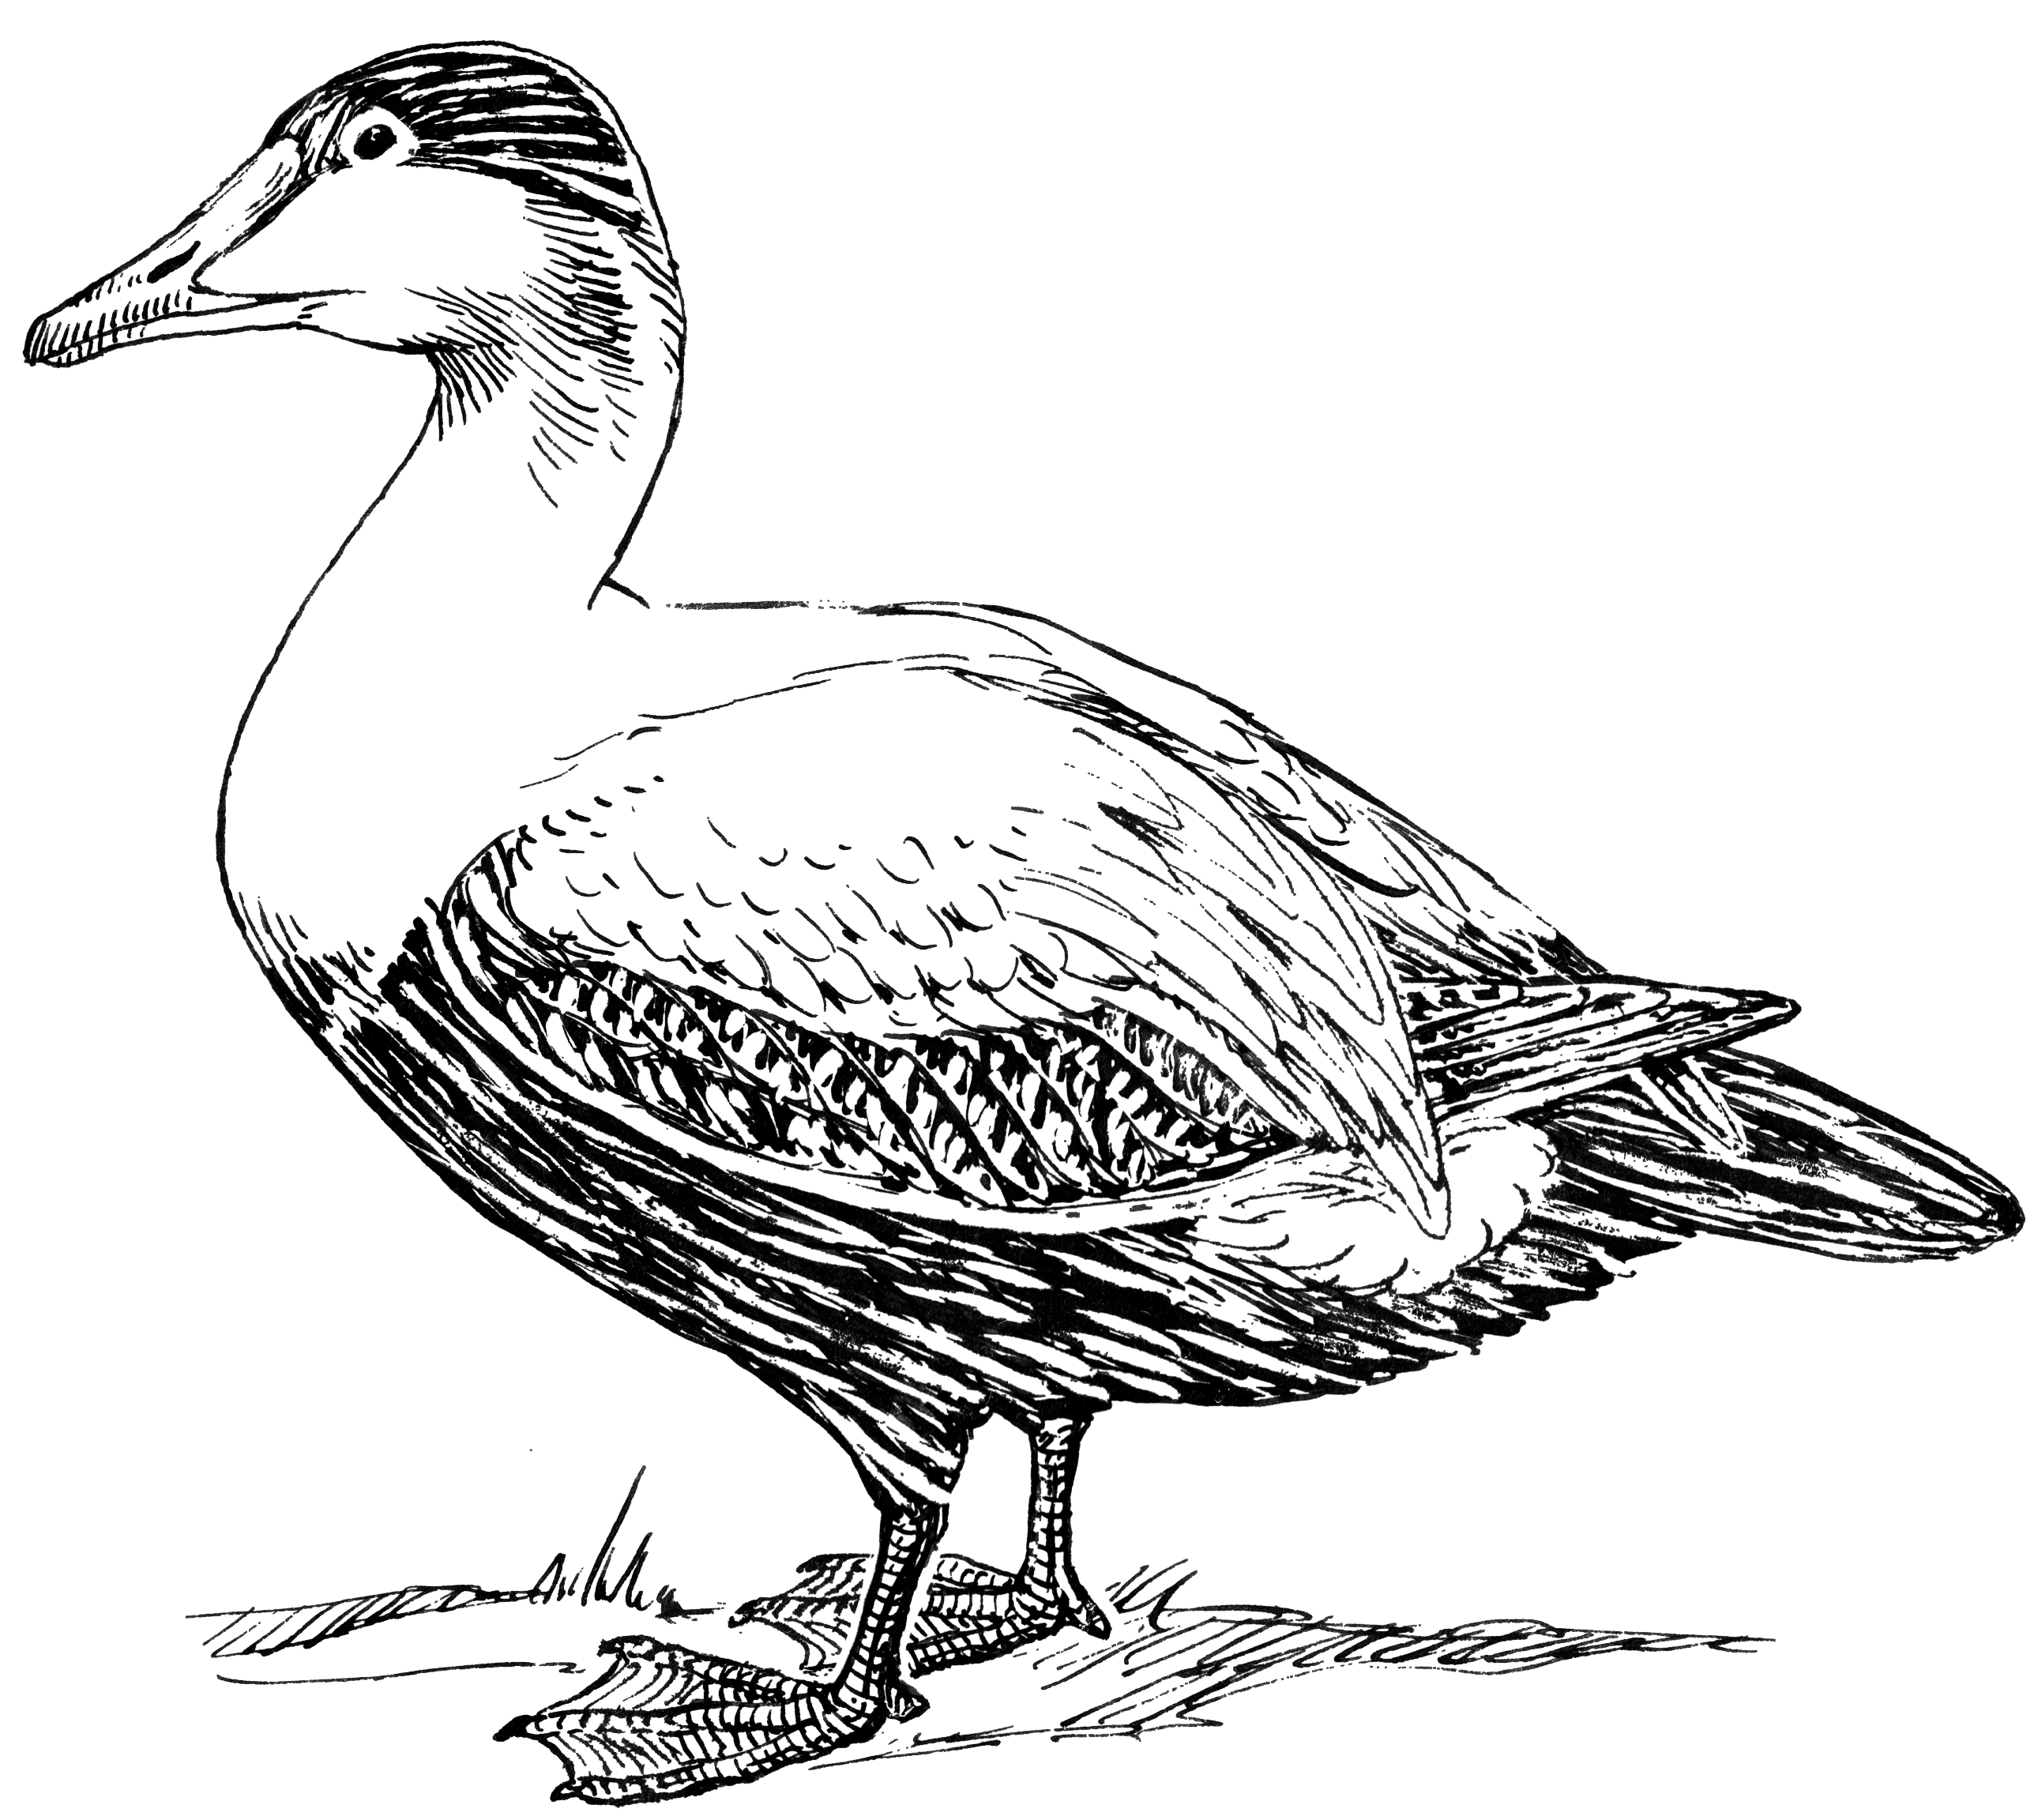
\includegraphics[width=.25\textwidth]{duck}
    
    \textit{If it looks like a duck and quacks like a duck\\ but it needs
    batteries,\\you probably have the wrong abstraction.}
  \end{center}
\end{frame}

\begin{frame}{Things that look like extensionality\dots}
  \begin{block}{Injectivity of constructors}
    \[
    succ(x) \neq succ(y) \lor x = y
    \]
    What happens if we treat this as an extensionality axiom?
  \end{block}
  
  \begin{block}{Solution}
    Exclude clauses with a disequality of the same sort as $x = y$
  \end{block}
\end{frame}

\begin{frame}{Things that look like extensionality\dots}
  \begin{block}{Axiomatization of arrays}
    \[
    i = j \lor select(store(a,i,e), j) = select(a, j)
    \]
  \end{block}

  \begin{block}{Solution}
    Exclude clauses with an equality other than the one among
    variables
  \end{block}
\end{frame}


\section{Results}
\begin{frame}{On 36 hard set theory problems}
  \begin{center}
    {\footnotesize
      \begin{tabular}{ccc}
        \hline\noalign{\smallskip}
        Prover & Logic & Solved \\
        \noalign{\smallskip}\hline\noalign{\smallskip}
        Vampire\textsuperscript{EX} & TFF & 36 \\
        Vampire\textsuperscript{EX} & FOF & 36 \\
        iProver & TFF & 16 \\
        Princess & TFF & 15 \\
        Princess & FOF & 15 \\
        Vampire & TFF & 14 \\
        Vampire & FOF & 13 \\
        CVC4 & FOF & 13 \\
        E & FOF & 11 \\
        Muscadet & FOF & 7 \\
        Zipperposition & FOF & 4 \\
        Beagle & TFF & 2 \\
        Beagle & FOF & 2 \\
        E-KR-Hyper & FOF & 0 \\
        \hline
      \end{tabular}
    }
  \end{center}
\end{frame}

\begin{frame}{On 278 array theory problems}
  \begin{center}
    {\small
      \begin{tabular}{cc}
        \hline\noalign{\smallskip}
        Prover & Solved \\
        \noalign{\smallskip}\hline\noalign{\smallskip}
        Z3 & 277 \\
        Vampire\textsuperscript{EX} & 154 \\
        Vampire & 107 \\
        E & 81 \\
        Beagle & 16 \\
        Zipperposition & 15 \\
        Princess & 10 \\
        iProver & 9 \\
        CVC4 & 8 \\
        E-KR-Hyper & 8 \\
        Muscadet & 4 \\
        \hline
      \end{tabular}
    }
  \end{center}
\end{frame}

\begin{frame}{On 7224 TPTP problems}
  \begin{center}
    {\footnotesize
      \begin{tabular}{lcc}
        \hline\noalign{\smallskip}
        Strategy & solved & uniquely solved \\
        \noalign{\smallskip}\hline\noalign{\smallskip}
        original & 4015 & 156 \\
        original + known & 3870 & 8 \\
        original + all & 3747 & 50 \\
        \hline
      \end{tabular}
    }
  \end{center}
  known + all: 84 uniquely solved problems, including 12 never solved
  before
\end{frame}


\section{Conclusions}
\begin{frame}{Conclusions}
  \begin{itemize}
  \item ``Domain-specific'' inferences are useful
  \item It is better to have strategies that solve new problems,
    rather than many problems
  \item Theory reasoning is not the exclusive territory of SMT solvers
  \end{itemize}
\end{frame}


\begin{frame}
  \begin{center}
    \Huge{Questions?}
  \end{center}
\end{frame}

\end{document}
